\author{Tevin Achong - 816000026, Jonathan Owen - 816001156}
\documentclass[a4paper, 12pt]{article}

\usepackage[left=2cm, right=2cm, top=2cm]{geometry}
\usepackage{color}
\usepackage{graphicx}
\usepackage{float}
\usepackage[colorlinks = true,
			urlcolor = blue]{hyperref}
\usepackage{tikz}
\usetikzlibrary{shapes, arrows}

%Specs for flowcharts%
\tikzstyle{workstation} = [ellipse, minimum width=3cm, minimum height=1cm, text centered, draw=black]
\tikzstyle{server} = [cylinder, minimum width=3cm, minimum height=1cm, text centered, draw=black]
\tikzstyle{cnode} = [tape, minimum width=3cm, minimum height=1cm, text centered, draw=black]
\tikzstyle{arrow} = [thick, ->, >=stealth]

\begin{document}
\pagenumbering{roman}
\title{
		\textbf{Course Code:} INFO3606\\
		\textbf{Course Title:} Cloud Computing\\
		\textbf{Semester Project}
		\date{April 15, 2020}
}
\maketitle

\newpage
\pagenumbering{arabic}

\tableofcontents

\newpage
\section{Group Member Roles and Responsibilities}
This group was comprised of Tevin Achong (816000026) and Jonathan Owen (816001156). Overall, the project was a highly collaborative effort. However, since there were many tools to be researched, we divided the work among both members. Tevin was responsible for the research and write up on the tools \textbf{Chef}, \textbf{Ansible}, and \textbf{Fuel}; while Jonathan was responsible for the research and write up on the tools \textbf{Puppet} and \textbf{Compass}. Both members collaborated to produce the table of comparisons seen at the end of the document.

\newpage
\section{Chef}
Chef is a configuration management tool that is used to streamline the task of configuring and maintaining a company's servers. Aditionally, Chef can integrate with various cloud-based platforms to automatically provision and configure new machines. It contains solutions for small and large scale systems, and features and pricing for each of the various ranges. Essentially, Chef ensures that the files and the software that users are expecting to be on a machine are actually present, configured correctly, and working as is expected. Performing these tasks for a single machine is fairly straightforward. However, as an organization's infrastructure scales up (more machines are introduced) it becomes increasingly difficult. This is the reason Chef was developed and is used.

\subsection{Components}
Chef operates with three core components: \textbf{Chef Server}, \textbf{Workstations}, and \textbf{Nodes}. These three components communicate in a linear fashion, as explained below. 
\begin{enumerate}
\item
\textbf{Workstations:} All the configuration code is created, tested, and changed at workstations, which are personal computers or virtual servers. There can exist as many workstations as is necessary. Additionally, cookbooks and policies that will be pushed to the Chef server and pulled by nodes are tested and maintained here. The Chef Workstation provides chef and command line tools, the testing tools Test Kitchen, ChefSpec, Cookstyle, and Foodcritic, and InSpec - a tool that allows you to write automated tests for compliance, security and policy requirements. Cookbooks created on workstations can be used privately or by one organization, or uploaded to the Chef Supermarket for other to use. Workstations can also be used to download cookbooks created by other Chef users and found in the Chef Supermarket.
\item
\textbf{Nodes:} These are the servers that are managed by Chef i.e. the machines to which changes are being pushed. Nodes are generally a fleet of multiple machines that require the benefits of automation. Chef can manage nodes that are virtual servers, containers, network devices, and storage devices and a Chef client is installed on every node that is under management by Chef. 
\item
\textbf{Chef Server:} The Chef Server is the center of all of Chef's operations. It provides a communication pathway between the workstations (where infrastructure is coded) and the nodes (where the configurations are deployed by the Chef client). Any configuration files, metadata, cookbooks and other information created on workstations are stored on the Chef server. Aditionally, the Chef server contains information regarding the state of all nodes at the time of the last chef-client run. Any changes made to infrastructure code must pass through the Chef server in order to be applied to nodes. Before accepting changes, the Chef server authenticates all communication via its REST API using public key encryption. In turn, the Chef Server is also made of several components which aid it in efficiently communicating with workstations and nodes. Each Chef Server uses an NGINX front-end load balancer to route all requests to the Chef Server API, and PostgreSQL to store data. A web interface, known as Chef manage, is used for common Chef server management tasks. An Apache Solr instance, wrapped by chef-solr, is used for indexing and searching. All these components help to make the Chef server capable of handling requests for several thousands of nodes and make Chef server a resource heavy application.
\end{enumerate}

\subsection{Architecture}
In order to achieve its goals, Chef treats infrastructure as code. Instead of manually changing anything, the machine setup is described in a Chef \textit{recipe}. \textit{Cookbooks} store collections of recipes. Ideally, one cookbook relates to a single task, but it can have numerous server configurations involved. The chef server stores each of the cookbooks and as a new chef client node checks in with the server, recipes are sent to tell the node how to configure itself. Afterwards, the client will occassionally check in with the server to see if anything needs to be changed. If something does need to be changed, then the client deals with it. Patches and updates can be applied to the entire infrastructure by changing the recipe; there is no need to interact with each machine individually.
\textit{Bookshelf} is used to store cookbooks and related files and templates. The Chef Server uses a Bookshelf that operates as a versioned repository. Full root access is required. Whenever a cookbook is uploaded to the Chef server, the new version of the cookbook is compared to the one already stored on the server. If any changes exist, a new version is stored. If resources are shared between cookbooks and cookbook versions, they will not be stored more than once. This is because the Chef Server stores one copy of a file or template.
As such, Chef utilizes a three-tier client-server architecture. The working units (like cookbooks) are developed on the Chef workstation. From the command line utilities like Knife, they are uploaded to the Chef server and all the nodes which are present in the architecture are registered with the Chef server. Figure 1 below depicts this architecture.\\

\begin{figure}[H] 
\begin{center}
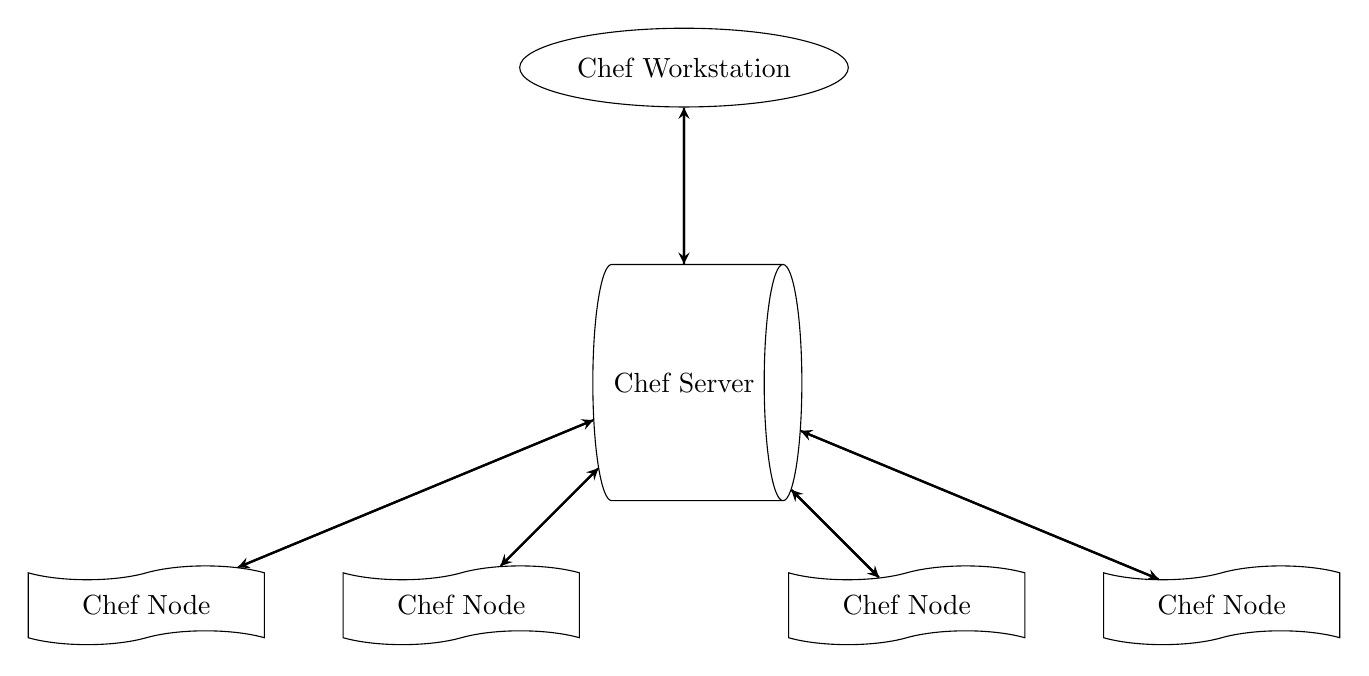
\begin{tikzpicture}[node distance=4cm]
\node (workstation) [workstation] {Chef Workstation};
\node (server) [server, below of=workstation] {Chef Server};
\node (cnode_one) [cnode, below left of=server] {Chef Node};
\node (cnode_two) [cnode, below right of=server] {Chef Node};
\node (cnode_three) [cnode, right of=cnode_two] {Chef Node};
\node (cnode_four) [cnode, left of=cnode_one] {Chef Node};

\draw [arrow] (workstation) -- node {} (server);
\draw [arrow] (server) -- node {} (workstation);

\draw [arrow] (cnode_one) -- node {} (server);
\draw [arrow] (server) -- node {} (cnode_one);
\draw [arrow] (cnode_two) -- node {} (server);
\draw [arrow] (server) -- node {} (cnode_two);
\draw [arrow] (cnode_three) -- node {} (server);
\draw [arrow] (server) -- node {} (cnode_three);
\draw [arrow] (cnode_four) -- node {} (server);
\draw [arrow] (server) -- node {} (cnode_four);

\end{tikzpicture}
\end{center}
\caption{Architecture of Chef} \label{fig:1}
\end{figure}

\newpage
\subsection{Features}
Chef provides the following features:
\begin{itemize}
\item
Automatic Backup
\item
Automatic Notifications
\item
Compliance Management
\item
Configuration Management
\item
Data Recovery
\item
Data Visualization
\item
Real Time Analytics
\item
Real Time Data
\item
Real Time Monitoring
\item
Real Time Notifications
\item
Real Time Reporting
\item
Real Time Updates
\item
Server Monitoring

\end{itemize}

\subsection{Official Website}
The official website for Chef is located at \href{https://www.chef.io}{https://www.chef.io}.
\subsection{Latest Version}
As of January 28, 2019, the latest stable release of the Chef client is v14.10.9.\\
As of October 15, 2018, the latest stable release of the Chef server is v12.18.14.
\subsection{Advantages}
Advantages of using Chef include:
\begin{enumerate}
\item
There is a low barrier for entry. Chef uses native Ruby language for configuration. This means that it can be easily picked up by anyone who has some development experience.
\item
It integrates execellently with cloud. Using the knife utility, Chef can be easily integrated with most existing cloud technologies. It is a suitable tools for organizations that wish to distribute their infrastructure on multi-cloud environment. 
\item
Chef can help organizations to accelerate software delivery, i.e. how quickly the software is able to be changed in response to new requirements or conditions. 
\item
Helps organizations to catch bugs and issues before they occur. Infrastructure automation increases a system's resiliency just as much as it accelerates delivery speed. 
\item
Improving risk management - the \textit{quality} of changes made to the software.
\item
When using Chef, you can deliver all your infrastructure everywhere continuously.
\end{enumerate}
\subsection{Disadvantages}
Some disadvantages include:
\begin{enumerate}
\item
Cookbooks require constant monitoring so that the people who are working do not cause any issues with them. 
\item
Only Chef solo is available. 
\item
Currently, Chef is only a good fit for Amazon Web Services Cloud. 
\item
Someone who is not familiar with Ruby may have a hard time learning it.
\item
There is currently a lack of proper documentation.
\end{enumerate}

\newpage
\section{Ansible}
Ansible is an open-source automation tool, or platform, used for IT tasks such as configuration management, application deployment, intraservice orchestration, and provisioning. Thus, simplifying complex tasks, making the jobs of developers more manageable and allowing them to focus attention on other tasks that addd value to their organization. 

\subsection{Components}
\begin{itemize}
\item
\textbf{Plays}\\
Playbooks contain plays. Plays are essentially groups of tasks that are performed on defined hosts to enforce your defined functions. Each play must specify a host or group of hosts. 
\item
\textbf{Tasks}\\
Tasks are actions carried out by playbooks. A task definition can contain modules such as yum, git, service, and copy.
\item
\textbf{Roles}\\
A role is the way Ansible bundles automation content to make it reusable. Roles are organizational components that can be assigned to a set of hosts to organize tasks. Therefore, instead of creating a monolithic playbook, we can create multiple roles, with each role assigned to complete a unit of work. For example: a webserver role can be defined to install Apache and Varnish on a specified group of servers.
\item
\textbf{Handlers}\\
Handlers are very similar to tasks. The major difference is that a handler will be executed only when it is called by an event. The handler is called by the [notify] directive. The name of the notify directive and the handler must be the same. 
\item
\textbf{Templates}\\
Templates files are based on Python's Jinja2 template engine and have a .j2 extension. If necessary, you can place contents of your index.html file into a template file. But the real power of templates is comes when variables are used. Ansible's [facts] can be used in template files, and users can even call custom variables.
\item
\textbf{Variables}\\
You can include custom-made variables in your playbooks. Variables can be defined in five (5) different ways:
\begin{enumerate}
\item
Variables defined under the vars\_file attribute.
\item
Variables defined in \textit{role}/vars/apache-install.yml
\item
Variables passed through the command line.
\item
Variables defined in the play under vars.
\item
Variables defined in group\_vars/ directory.
\end{enumerate}
\end{itemize}

\subsection{Architecture}
The architecture that makes up Ansible is as follows:
\begin{itemize}
\item
\textbf{Modules}\\
Ansible works by connecting to your nodes and pushing out small programs, called "Ansible Modules" to them. These programs are written to be resource of the desired state of the system. Ansible then executes these modules (over SSH by default), and removes them when finished. Your library of modules can reside on any machine, and there are no servers, daemons, or databases required. Typically you'll work with your favorite terminal program, a text editor, and probably a version control system to keep track of changes to your content.
\item
\textbf{Plugins}\\
Plugins are pieces of code that augment Ansible's core functionality.
\item
\textbf{Inventory}\\
The inventory is a configuration file where you define the host information.
\item
\textbf{Playbooks}\\
A playbook is where users define how to apply policies, declare configurations, orchestrate steps and launch tasks either synchronously or asynchronously on their servers.  Each playbook is composed of one or more plays. Playbooks are normally maintained and managed in a version control system like Git. They are expressed in YAML (Yet Another Markup Language). In most cases - especially in enterprise environments - using Ansible playbooks is recommended.
\end{itemize}


\subsection{Features}
\begin{itemize}
\item
\textbf{Configuration Management}\\
Ansible is designed to be very simple, reliable, and consistent for configuration management. Users who are familiar with the field of Information Technology can usually get up and running fairly quickly with Ansible. Ansible configurations are simple data descriptions of infrastructure and are both by readable by humans and parsable by machines. A password or an SSH key is all that is needed to start managing systems. For example, if a user wants to install an updated version of a specific type of software on all the machines in their enterprise, all they need to do is write out all the IP addresses of the nodes (also called remote hosts) and write an Ansible playbook to install it on all the nodes, then run the playbook from their control machine.
\item
\textbf{Application Deployment}\\
Ansible also allows users to quickly and easily deploy multitier applications. Users do not need to write custom code to automate their systems; they simply need to list the tasks required to be done in a playbook, and Ansible will figure out how to get their systems to the state they want them to be in. In other words, users need not configure the applications on every machine manually. When a playbook is run from the user's control machine, Ansible uses SSH to communicate with the remote hosts and run all the commands (tasks).
\item
\textbf{Orchestration}
Orchestration involves bringing different elements into an efficiently-running, whole operation. For example, with application deployment, users need to manage the front-end and backend services, databases, networks, storage, and so on. They also need to ensure that all tasks are handled in the proper order. Ansible uses automated workflows, provisioning, and more to simplify the process of orchestration. Once the infrastructure has been defined using Ansible playbooks, that same orchestration can be used wherever it is needed. This is due largely to the portability of Ansible playbooks.
\item
\textbf{Security and Compliance}\\
As with application deployment, sitewide security policies (such as firewall rules) can be implemented along with other automated processes. If the security details on the control machine are configured and the associated playbook is run, all the remote hosts will automatically be updated with those details. Therefore, users will not need to monitor each machine for security compliance continually manually. For extra security, an admin's user ID and password are not retrievable in plain text on Ansible.
\item
\textbf{Cloud Provisioning}\\
The first step in automating your applications' life cycle is automating the provisioning of your infrastructure. With Ansible, you can provision cloud platforms, virtualized hosts, network devices, and bare-metal servers.
\end{itemize}

\subsection{Official Website}
The official website for Ansible is \href{https://www.ansible.com/}{https://www.ansible.com/}.
\subsection{Latest Version}
As of June 14, 2018, the latest version of Ansible is 2.9.
\subsection{Advantages}
Ansible offers the following advantages:
\begin{enumerate}
\item
\textit{Free:} Ansible is an open-source tool.
\item
\textit{Very simple to set up and use:} No special coding skills are necessary to use playbooks in Ansible.
\item
\textit{Powerful:} Ansible lets you model highly complex IT workflows.
\item
\textit{Flexible:} The entire application environment can be orchestrated no matter where it is deployed. It can also be customized to suit user's needs.
\item
\textit{Agentless:} No other software or firewall ports need to be installed on the client systems users wish to automate. Setting up a separate management structure is also unnecessary. 
\item
\textit{Efficient:} Because there is no need to install any extra software, there is more room for application resources on the server.
\end{enumerate}
\subsection{Disadvantages}
Disadvantages of Ansible include:
\begin{enumerate}
\item
\textbf{No Notion of State:} Unlike comparable automation tools, Ansible has no notion of state. Since it does not keep track of dependencies, the tool simply executes a sequential series of tasks, stopping when it finishes, fails or encounters an error. Many users tend to prefer that their automation tool maintain an extensive catalog for ordering, allowing them to reach a defined state regardless of any variance in environmental conditions.
\item
\textbf{Nascent Windows Support}: Ansible suports both Unix/Linux and Windows nodes. For Windows nodes it uses native powershell remoting (as opposed to SSH), and a Linux control machine is still required for managing Windows hosts. Ansible is still early in its efforts to extend support for Windows. 
\item
\textbf{Minimal Enterprise Support Experience:} Ansible has had considerably less experience working with large enterprises than competitors like Chef and Puppet. 
\item
\textbf{Relatively New:} Ansible has not been around as long as competitors such as Chef or Puppet. As a result, it has the smallest developer/user community and has the least easily accessible material on the internet for self-help and troubleshooting. Less time on the market means more bugs, edge scenarios, and software issues have perhaps not yet appeared. 
\end{enumerate}


\newpage
\section{Fuel}
Fuel is an open-source deployment and management tool for OpenStack. It was developed as an OpenStack community effort, and provides an intuitive, GUI-driven experience for deployment and management of OpenStack and related community projects and plug-ins.
Fuel provides consumer-grade simplicity to streamline and accelerate the otherwise time-consuming, often complex, and error-prone process of deploying, testing and maintaining various configuration flavors of OpenStack at scale. Unlike other platform-specific deployment or management utilities, Fuel is an upstream OpenStack project that focuses on automating the deployment and testing of OpenStack and a range of third-party options, so it is not compromised by hard bundling or vendor lock-in.
\subsection{Components}


\subsection{Architecture}
Fuel is comprised of several independent components. Some components are Fuel-specific components, while others are third-party services like Cobbler, Puppet, Mcollective, etc. Some components can be reused separately from Fuel without any further modifications, while some others will require small adjustments.
\begin{itemize}
\item
\textbf{UI} is single page application, and is written in JavaScript. It uses bootstrap and backbone frameworks.
\item
\textbf{Nailgun} is the core of the Fuel project. Like other OpenStack projects, Nailgun is written in the Python programming language. It implements a REST API as well as deployment data managemen. It manages disk volumes, configuration data, network configuration data and any other environment specific data which are necessary for successful deployment. It has required orchestration logic to build isntructions for provisioning and deployment in the right order. Nailgun uses a SQL database to store its data and AMQP service to interact with workers. 
\item
\textbf{Astute} represents Nailgun's workers, and its function is to run certain actions according to the instructions provided by Nailgun. Astute is nothing more than a layer which encapsulates all the details with a variety of services such as Cobbler, Puppet, shell scripts etc. and provides a universal asynchronous interface to those services. We can either manage a service directly via its native protocol or we can use MCollective agents to perform specific tasks. Astute exchanges the data with Nailgun via AMQP. 
\item
\textbf{Cobbler} is currently used as a provisioning service. There is a POC ready to move to Ironic, and a production version is being implemented. 
\item
\textbf{Puppet} is currently Fuel's only deployment service. It would be possible to create MCollective agents to manage other configuration management frameworks, such as Chef or SaltStack. 
\item
\textbf{MCollective agents} enable us to perform specific tasks such as hard-drive cleaning, network connectivity probing, etc. 
\item
\textbf{OSTF(OpenStack Testing Framework)} is a separate component which can be easily removed and reused without Fuel. It implements post-deployment verification of OpenStack. Its main goal is to verify maximum functionality taking a minimum amount of time.
\end{itemize}

\begin{figure}[H]
	\centering
	\includegraphics[width=\linewidth]{img/fuel_arch.png}
  	\caption{The Architecture of Fuel (source: \href{https://wiki.openstack.org/wiki/Fuel}{https://wiki.openstack.org/wiki/Fuel})}
	\label{fig:4-waycache}
\end{figure}


\subsection{Features}
The key features of Fuel are:
\begin{itemize}
\item
hardware discovery
\item
hardware configuration in UI (networks \& disk partitioning)
\item
ability to spin up and manage multiple OpenStack clusters
\item
support for non-HA and HA OpenStack deployment configurations
\item
pre-deployment checks and network validation
\item
post-deployment checks and running a set of tests for validating deployed OpenStack
\item
view logs in real-time through UI
\item
support for CentOS and Ubuntu, and it can be extended to support other distributions too
\item
support for multiple OpenStack distributions
\end{itemize}

\subsection{Official Website}
The official documentation for Fuel can be found at \href{http://docs.fuel-infra.org/openstack/fuel/}{http://docs.fuel-infra.org/openstack/fuel/}.
\subsection{Latest Version}
Based on our research, the latest available version of Fuel for OpenStack is 9.1.
\subsection{Advantages}
\subsection{Disadvantages}

\newpage
\section{Puppet}
Puppet is a powerful enterprise-grade Configuration Management tool that is used for deploying, configuring and managing servers. Puppet uses a Ruby-based domain specific language (DSL) reducing the complexity of automation for engineers trying to complete basic tasks. Furthermore Puppet focuses on automation, “write once deploy many” code and auditing and enforcing code.

\subsection{Components}
Puppet environment consist of two main components and they are the main server environment called the puppet master and the client environment called the Puppet client. Within these:
\begin{itemize}
\item
Puppet master - Puppet Master is the main mechanism that handles all the configurations. The master applies the configurations to nodes using the Puppet agent.
\item
Puppet Agent - Puppet Agents are the working machines which are managed by the Puppet master. The Puppet agent daemon service running inside them.
\item
Config Repository - This is the repository where all nodes and server related configurations are saved and pulled when required.
\item
Facts - This  is all the information related to the node or the master machine. They are used for analyzing the current status of any node. On the basis of facts, changes are done on any target machine. There are pre-defined and custom facts in Puppet.
\item
Catalog - All the manifest files or configuration which are written in Puppet are first converted to a compiled format called catalog and later those catalogs are applied on the target machine.
\item
Manifests - These are the authentic codes for configuring the clients.
\item
Class - Classes properly organize the code. 
\item
Resources - Within the coding block resources may represent packages, files, users and commands.
\item
Nodes - Nodes are considered to be all servers or clients that need to be managed.
\item
Puppet client - The Puppet client is the machine that is configured, it consist of the Agent and Facter. The agent constantly interacts with the master server to guarantee that the certificates are being updated appropriately. The facter collects the current state of the client that is used and communicates it back through the agent.

\end{itemize}


\subsection{Architecture}
How Puppet executes its operations:\\
Firstly an agent node sends facts to the master and requests a catalog. Secondly the puppet master server compiles and returns the node’s catalog using the sources of information the master has access to.
Thirdly the puppet agent applies the catalog to the node by analyzing each resource the catalog describes. If resources are found not in their desired state, it makes the necessary changes to correct them. Or, in no-op mode, it examines what changes would be needed to reconcile the catalog.
Lastly the agent sends a report back to the puppet master.

\begin{figure}[H]
	\centering
	\includegraphics[width=\linewidth]{img/puppet_arch.jpg}
  	\caption{Puppet Architecture (\href{https://www.tutorialspoint.com/puppet/puppet\_architecture.htm}{https://www.tutorialspoint.com/puppet/puppet\_architecture.htm})}
	\label{fig:puppet_arch}
\end{figure}


\subsection{Features}
Puppet provides the following features:
\begin{itemize}
\item
Continuous Delivery
\item
Continuous Compliance
\item
Incident Remediation
\item
Configuration Management
\item
DevOps automation for a multi-cloud world
\end{itemize}

\subsection{Official Website}
The official website for Puppet is located at \href{https://puppet.com}{https://puppet.com}

\subsection{Latest Version}
As of March 10, 2020, the latest stable relase of Puppet management tool is Puppet 6.14.0.

\subsection{Advantages}
Advantages of using Puppet include:
\begin{enumerate}
\item
Puppet is open-source and it is also extendable. It can be extended to build custom libraries and modules to suit the needs of projects.
\item
Puppet allows resource abstraction. Configuration tasks that are done may be needed across a range of servers that all have different operating systems and other platform specific identities and administrators may not remember what was previously done. This is where factor helps Puppet know the system details such as the operating system and IP address. With this information, Puppet achieves abstraction.
\item
Puppet does transactions only if needed with the feature idempotency. This applies changes only when asked. If changes are already done to the system, puppet leaves the system at its present state.
\item
Puppet improves manageability and productivity for system administrators. They are freed up to focus on more complex tasks that require human intervention. Furthermore it helps the server become more manageable.
\item
Puppet is cross-platform allowing users to cover a wider range of platforms which makes more servers come into the configuration fold. Puppet operates on platforms such as Fedora, RHEL, Debian, Gentoo, Solaris, OS X, and Windows.
\item
Puppet declarative language is clean and easily to learn. Individuals with limited programming knowledge/skill can easily pick it up.
\item
Puppet has cron-like support, this schedule specific maintenance actions on a periodic basis. Furthermore helps the administrators accomplish some cron jobs in the maintenance cycle.
\item
Puppet has override mechanisms to override an instruction with another one for different scenarios. When exceptions are to be made while applying configurations the override mechanism is useful. 
\item
Puppet has an active community with plenty of active discussion boards, forums and experts always willing to assist individuals.
\end{enumerate}

\subsection{Disadvantages}
Disadvantages of using Puppet include:
\begin{enumerate}
\item
Puppet releases new versions rapidly making it a task to keep up with the new features and breaking changes.
\item
Puppet may not be suitable for smaller setups and businesess.
\item
Puppet does not have comprehensive reporting features.
\end{enumerate}

\newpage
\section{Compass}
Compass is an open source project for the automated deployment and management of OpenStack. It follows the OpenStack community four opens: Open Source, Open Community, Open Development, and Open Design. Furthermore it provides data modeling, configuration API, and WebUI to the end users in bootstrapping and manages a software defined data center infrastructure.

\subsection{Components}
Components in Compass include:
\begin{itemize}
\item
A RESTful API server which is implemented in Python Flask.
\item
A demo Web UI which consumes the RESTful APIs. This is a pure JavaScript WebApp developed with AngularJS. Furthermore it allows third party application to have a different UI using the same APIs.
\item
A meta-data module that developers use to provide custom data model for OpenStack configurations and expand core functionality. Also based on the metadata the RESTful API layer provides the updated API automatically and no code change is required.
\item
An adapter interface for automatic resource discovery. Current discovery mechanism is based on stanard MIB over SNMP query to ToR switches. Other mechanisms (such as IPMI, or Intel's next-gen RSA) are possible by adding plugins.
\item
An adapter interface for configuration management tools such as Chef  and Ansible . Other mechanisms (such as Puppet) are possible by adding plugins.
\item
A Cobbler interface for Operating system (OS) provisioning. Configuration details of kickstart files or seed files are hidden so the interface provides a user-friendly OS-level provisioning
\end{itemize}

\subsection{Architecture}

\begin{figure}[H]
	\centering
	\includegraphics[width=\linewidth]{img/compass_arch.png}
  	\caption{Compass Architecture}
	\label{fig:compass_arch}
\end{figure}

Compass provides programmability allowing easy integration with operators’ OSS and other ecosystem tools. It also enables extensibility through meta-data allowing specification of a different flavor of OpenStack configuration. Furthermore the plugins support also allows users to extend the system.

\subsection{Features}
Features of Compass:
\begin{itemize}
\item
Assisting systems administrators in determining hardware.
\item
Assisting systems administrator in deploying the OS and hypervisor.
\item
Implementation of different configuration flavors through metadata.
\item
Blending with other tools for resource discovery, OS planning, and package deployment
\end{itemize}

\subsection{Official Website}
The official website for Compass is located at \href{http://www.syscompass.org/}{http://www.syscompass.org/}.

\subsection{Latest Version}
As of Monday 21st March 2016 the latest release of compass is v2.5.

\subsection{Advantages}
Advantages of using Compass:
\begin{enumerate}
\item
Reduces the complexity and error-prone deployment process of several distributed systems for example Openstack and Ceph.
\item
Can remotely install and configure physical servers in the datacenter.
\item
Reduces the amount of time taken by datacenter server management 
\item
Can remotely install and configure a Hadoop cluster.
\item
Supports in bootstrapping the server pool correlated with any cloud platform from exposed metal nodes.
\item
The extensible architecture allows easy integration with most of the popular automation tools.
\end{enumerate}

\subsection{Disadvantages}

\section{Table of Comparison of Tools}
\begin{figure}[H]
	\centering
	\includegraphics[width=\linewidth]{img/table_comp.png}
  	\caption{Table of Comparison of Features}
	\label{fig:table_comp}
\end{figure}

\newpage
\section{References}
SHADOW SOFT\\
\textit{6 Benefits of Chef's Infrastructure Automation Tools}\\
Published on April 3, 2017\\
\href{https://shadow-soft.com/chef-benefits/}{https://shadow-soft.com/chef-benefits/}\\

\noindent
TUTORIALSPOINT\\
\textit{Learn Chef: absolute beginners}\\
\href{https://www.tutorialspoint.com/chef/chef_overview.htm}{https://www.tutorialspoint.com/chef/chef\_overview.htm}\\

\noindent
LINODE\\
\textit{A Beginner's Guide to Chef}\\
Published on December 18, 2019\\
\href{https://www.linode.com/docs/applications/configuration-management/beginners-guide-chef/}{https://www.linode.com/docs/applications/configuration-management/beginners-guide-chef/}\\

\noindent
SIMPLILEARN\\
\textit{What is Ansible: Advantages, Features, and Architecture}\\
Published on April 8, 2020 by Shivam Arora\\
\href{https://www.simplilearn.com/what-is-ansible-article}{https://www.simplilearn.com/what-is-ansible-article}\\

\noindent
CLOUDACADEMY\\
\textit{Ansible and AWS: Cloud IT Automation Management}\\
Published on October 21, 2015 by Chandan Patra\\
\href{https://cloudacademy.com/blog/ansible-aws/}{https://cloudacademy.com/blog/ansible-aws/}\\

\noindent
ANSIBLE\\
\textit{Ansible Architecture}\\
\href{https://docs.ansible.com/ansible/latest/dev_guide/overview_architecture.html}{https://docs.ansible.com/ansible/latest/dev\_guide/overview\_architecture.html}\\

\noindent
OPENSTACK WIKI\\
\textit{Fuel for OpenStack}\\
\href{https://wiki.openstack.org/wiki/Fuel}{https://wiki.openstack.org/wiki/Fuel}\\

\noindent
PUPPET\\
\href{https://puppet.com/}{https://puppet.com/}\\

\noindent
QUORA\\
\textit{What is the use of puppet?}\\
Published on August 30, 2016 by Karim Memon\\
\href{https://www.quora.com/What-is-the-use-of-puppet}{https://www.quora.com/What-is-the-use-of-puppet}\\

\noindent
PUPPET\\
\textit{Puppet Architecture}\\
\href{https://puppet.com/docs/puppet/latest/architecture.html}{https://puppet.com/docs/puppet/latest/architecture.html}\\

\newpage
\noindent
EZEELIVE\\
\textit{What is the Puppet? Its Pros and Cons}\\
Published on January 9, 2020.\\
\href{https://ezeelive.com/puppet-pros-cons/}{https://ezeelive.com/puppet-pros-cons/}\\

\noindent
OPENSTACK WIKI\\
\textit{Compass for OpenStack}\\
\href{https://wiki.openstack.org/wiki/Compass}{https://wiki.openstack.org/wiki/Compass}\\

\noindent
OPENDEV\\
\textit{Automating Distributed System Deployment to Baremetal Resources: compass-core}\\
\href{https://github.com/openstack/compass-core}{https://github.com/openstack/compass-core}\\

\noindent
OPENDEV\\
\textit{A web-based UI consuming the Restful API service provided by Compass}\\
\href{https://opendev.org/x/compass-web}{https://opendev.org/x/compass-web}\\

\noindent
GEEKFLARE\\
\textit{Top 5 Open Source Tools to Manage OpenStack Server}\\
Published on November 8, 2019\\
\href{https://geekflare.com/openstack-opensource-tools/}{https://geekflare.com/openstack-opensource-tools/}\\

\end{document}